\title{Quantifying the precision of decoding models for high-dimensional stimuli}
\author{Charles Zheng and Yuval Benjamini}
\date{\today}

\documentclass[12pt]{article} 

% packages with special commands
\usepackage{amssymb, amsmath}
\usepackage{epsfig}
\usepackage{array}
\usepackage{ifthen}
\usepackage{color}
\usepackage{fancyhdr}
\usepackage{graphicx}
\usepackage{mathtools}
\usepackage{csquotes}
\definecolor{grey}{rgb}{0.5,0.5,0.5}

\begin{document}
\maketitle

\newcommand{\tr}{\text{tr}}
\newcommand{\E}{\textbf{E}}
\newcommand{\diag}{\text{diag}}
\newcommand{\argmax}{\text{argmax}}
\newcommand{\Cov}{\text{Cov}}
\newcommand{\Var}{\text{Var}}
\newcommand{\argmin}{\text{argmin}}
\newcommand{\Vol}{\text{Vol}}
\newcommand{\comm}[1]{}
\newcommand{\indep}{\rotatebox[origin=c]{90}{$\models$}}
\newcommand{\Cor}{\text{Cor}}
\newcommand{\bx}{\boldsymbol{x}}
\newcommand{\by}{\boldsymbol{y}}
\newcommand{\bX}{\boldsymbol{X}}
\newcommand{\bY}{\boldsymbol{Y}}
\newcommand{\bS}{\boldsymbol{S}}
\newcommand{\bu}{\boldsymbol{u}}
\newcommand{\bv}{\boldsymbol{v}}
\newcommand{\bU}{\boldsymbol{U}}
\newcommand{\bV}{\boldsymbol{V}}
\newcommand{\bB}{\boldsymbol{B}}
\newcommand{\bepsilon}{\boldsymbol{\epsilon}}

\begin{abstract}
The analysis of encoding and decoding models is a common theme in both
cell recording studies and in neuroimaging.  A basic measure of the
precision of a decoder is its accuracy at distinguishing $k$ different
stimuli. However, the fixed-$k$ accuracy becomes insensitive beyond
limited range of precision: low-precision decoders saturate at the
chance accuracy $1/k$, while high-precision decoders saturate near
perfect accuracy.  On the other hand, the entire curve of accuracies
for $k = 2,3,...$ provides a detailed and interpretable
characterization of decoder performance.  However, due to limited
sampling, usually only a portion of the curve can be estimated:
furthermore, it is unclear how to summarize the information in the
curve by a single statistic.  We show that under a high-dimensional
limits, the mutual information becomes a sufficient statistic for
reconstructing the entire accuracy curve, therefore suggesting the
adoption of the mutual information as measure of decoder precision.
Based on our theory, we develop a novel estimator of mutual
information suited for high-dimensional settings (such as those found
in neuroimaging), and also a procedure for extrapolating the accuracy
curve to arbitrarily many stimuli.
\end{abstract}


\section{Introduction}
Both computational and cognitive neuroscience are concerned with
understanding brain function: while computational neuroscience is
concerned with understanding functionality at the level of the spiking
behavior of individual neurons and small neural populations, cognitive
neuroscience tends to emphasize functionality at the level of
macroscale regions of the interest in the brain.  While the recording
technologies, motivating questions, and analytical methodologies
differ between the two subdisciplines, the conceptualization of brain
functionality in terms of \emph{encoding} and \emph{decoding} models
has been widely applied in both
areas \cite{QuianQuiroga2009}\cite{Naselaris2011}.  In computational
neuroscience, cell recording experiments are conducted to determine
whether spike trains have a temporal and/or correlational
code \cite{Nelken2005}\cite{Hatsopoulos1998}, to examine how the
neural code adapts to changes in stimulus
distribution \cite{Fairhall2001} and whether downstream neurons make
use of higher-order correlations for decoding \cite{Oizumi2010}.
Meanwhile, in neuroimaging studies, functional MRI experiments are
employed to model the receptive fields of early visual areas in the
human brain \cite{Kay2008a}, to examine the semantic encoding of words \cite{Mitchell2008}
or objects \cite{Huth2012}.

The dual perspectives of encoding and decoding originate naturally
from the fact that in examining the link between brain activity and
function, one can either start with brain activity on one end, or with
external stimulation or behavioral observation on the other end.
Starting by exposing the subject to sensory stimuli or prompting the
subject to engage in particular motor tasks, one can search for areas
in the brain which respond to the task: in other words, one can test
to see which areas of the brain \emph{encode} the given stimulus.  In
the other direction, one seeks to understand the functionality of a
given brain region: in other words, how to \emph{decode} brain
activity in that region.

Formulation of encoding models is relatively straightforward, since
one needs only to characterize the observed brain response to a given
stimulus.  One can further ask how to distinguish between signal and
noise in the encoding mechanism \cite{Nelken2005}, or in complex
stimuli, seek a linearizing feature set which reveals the nature of
the brain representation \cite{Naselaris2011}.  However, the
establishment of complete decoding models is much less amenable to
experiemental manipulation, since to exhaustively characterize the
functionality of a neuron, one would have to know in advance the type
of information it encodes.  Early advances in decoding often depended
on strokes of luck: Hubel \cite{Hubel1982} originally discovered the
existence of neurons with orientation-sensitive receptive fields due
to the vigorous response of a cell to the perfectly angled shadow of a
glass slide that they were inserting into the ophthalmoscope.  Yet,
even now, the goal of completely characterizing the function of a
given brain region remains a difficult task, with the most promising
approach being a \emph{reverse inference}
procedure \cite{Poldrack2006} which aggregates information from the
literature about activity-functionality relationships.

A more feasible goal is to establish the \emph{precision} with which a
neuron can decode a particular type of feature.  This can be
accomplished by first training an encoding model, and then inverting
the encoding model using Bayes' rule to obtain a decoding
model \cite{Oram1998}\cite{QuianQuiroga2009}\cite{Naselaris2011}.  

By decoding \emph{precision}, we mean the specificity which we can
identify or reconstruct the stimulus based on the neural response.  As
such, in our view, the term decoder \emph{precision} is more or less
synonymous with terms such as decoder \emph{performance} or
decoder \emph{accuracy} as they are used in the literature.  However,
we choose the word \emph{precision} in particular, because it
communicates the idea that the essential quality of a good decoder is
that it allows one to confidently and precisely infer the stimulus.

Measures of decoding precision can be used to support several
different kinds of scientific inferences.  When there exist multiple
plausible encoding models--for instance, a model where stimulus
information is encoded solely by average firing rate versus a model
where inter-spike timings also carry information--the precision of the
decoder can be used as a basis for deciding the best encoding model.
For two encoding models with equal complexity, such as comparing two
different types of receptive field models, the model with better
decoding precision could be considered the more plausible model.  In
the case where a more complex encoding model is compared to a strictly
simpler model--such as comparing a model with a temporal code versus a
model only incorporating average firing rate, a substantial
improvement in decoding precision for the more complex model is needed
to demonstrate its validity, since in the null hypothesis where the
simpler model is correct, the more complex model should still have
approximately equal decoding performance.

Yet another application of decoding precision is to track the
adaptivity of the neural code.  Fairhall \cite{Fairhall2001} recorded
the output of a motion-sensitive neuron in a fly in response to a
visual stimulus with changing angular velocity.  Changing the variance
of the stimulus results in rapid adaptation: the neural code starts
adapting to the change in stimulus distribution within tens of
milliseconds, which is reflected by an increased or decreased
precision (as measured by mutual information) in resolving angular
velocity to match the variance of the stimulus.  More generally,
comparisons of decoding precisions between different conditions can
show how the encoded information increases or decreases across
experimental conditions.  Kayser \cite{Kayser2010} demonstrated how
the mutual information between a sound stimulus and neurons in the
auditory cortex increased when the subjects were also presented a
matching visual stimulus (e.g. showing a picture of a lion roaring
while playing the sound of a lion's roar.)

Differing types and parameterizations of stimuli naturally lead to
differing measures of decoding precision.  For stimuli which can be
parameterized by a scalar $x$, the precision can be measured by the
squared correlation coefficient $R^2$ \cite{Abbott1994}.  However, the
resulting measure of precision is not invariant to scaling of the
parameterization: for instance, the choice of whether to parameterize
volume on an absolute scale or a logarithmic scale.  The mutual
information \cite{Shannon1948} between the stimulus and the predicted
stimulus is invariant to the parameterization of the stimulus.  Due to
its invariance and a number of other properties, the mutual
information is widely used to measure the precision of the neural code
in cell recording studies, both for single-neuron decoding
models \cite{Borst1999} and for population coding
models \cite{QuianQuiroga2009}\cite{Ince2010}.

However, the difficulties of estimating mutual information in small
samples has been widely recognized, with a large literature on bias
correction methods \cite{Panzeri2007}\cite{Paninski}.  Methods for
bias correction have been developed for three different sample size
regimes: the moderate-sample regime, where the number of observations
is larger than the number of stimulus-response
pairs\cite{Miller1955}\cite{Strong1998}\cite{Treves1995}, the
undersampled regime, where the number of observations is less than the
number of stimulus-response pairs \cite{Nemenman2004}, and
a \emph{stimulus-undersampled} regime, where only a small fraction of
possible stimuli are sampled, but with a large number of observations
for each of the sampled stimuli \cite{Gastpar2009}.  Nevertheless,
even the bias-corrected estimates may be unusably inaccurate in
problems of moderate dimensionality, since the cardinality of response
space grows exponentially with the dimensionality.  In such cases,
alternative approaches for estimating the mutual information include
the assumption of a parametric model \cite{Brunel1998}\cite{Gastpar2009}\cite{Yarrow2012}, or usage of
the maximum entropy principle to obtain bounds on the mutual
information subject to the empirical moments of a certain
order \cite{Ince2009}\cite{Globerson2009}.

Perhaps due to the technical difficulties of estimating mutual
information in high dimensions, mutual information has never, to our
knowledge, been used as a measure of decoding precision in
neuroimaging studies, although it has been proposed for the purpose of
bypassing the modelling of the hemodynamic response function for
single-voxel analyses \cite{FuhrmannAlpert2007}.  Instead, a variety
of methods are employed to characterize the precision of decoding
models, depending on the nature of the stimulus and the experimental
setup.

In task fMRI experiments where stimuli are drawn from a number of
disjoint semantic categories-- for instance, `birds', `insects', and
`mammals' as in \cite{Connolly2012}, it is natural to construct a
decoder which outputs the predicted category of a stimulus as a
function of the response.  Such a decoder is known as
a \emph{classifier} in the machine learning
literature \cite{Hastie2009a}, and a natural measure of classifier
precision is the probability that the decoder outputs the correct
category on a new, randomly drawn test example, which is
the \emph{classification accuracy}.

In experiments where the subject is presented a number of
parameterized stimuli are drawn from a continuous distribution (such
as natural images or sounds), there are two types of decoders which
can be constructed.  In the first case, one constructs a decoder which
estimates the parameters of the stimulus which we call
a \emph{reconstructor}: the precision of such a decoder is measured by
the correlation between the estimated and true parameter vector
\cite{Pasley2012} \cite{Nishimoto2011}\cite{Naselaris2009}.
In the second case, one constructs a decoder which picks the most
likely stimulus from a finite library of examples \emph{which includes
the true stimulus} \cite{Kay2008a}\cite{Mitchell2008}.  Since the true
stimulus is included in the library, the task is to `identify' the
correct stimulus from the library.  A natural measure of decoder
performance is therefore the probability of correct identification.
However, note that this probability is dependent on the arbitrary
choice of the size of the exemplar library: a different choice for
library size therefore results in a different measure of precision.
We refer to the probability of correct classification for a library of
$k$ exemplars as the \emph{$k$-example identification accuracy}.

In their respective domains, these different measures of precision
suffice to make inferences on many interesting scientific questions:
to list a few examples, showing the superiority of a Gabor filters
versus center-surround filters for modeling the receptive fields of V1
and V2 neurons \cite{Kay2008a}, or demonstrating that brain activity
in response to viewing an Engish noun can be predicted from word
association frequencies \cite{Mitchell2008}.  

A commonality to all applications of decoding models in neuroimaging
is the pairwise comparison of two decoding models (Gabor
vs. retinotopic) or the comparison of a single decoding model to
chance accuracy.  Looking ahead to anticipate what kinds of analyses
might be employed in the future based on neuroimaging data, it is
suggestive to note that the earliest decoding studies in the cell
recording literature also involved comparisons between two or three
different decoders \cite{Eckhorn1976}.  However, as neuroscientists
began to consider questions of population coding, analyses of the
redundancy between neurons started to make use of comparisons between
large numbers of decoders: for a population of $N$ neurons, one might
compare the precision of a decoder (mutual information) based on the
entire ensemble, compared to the precisions of decoders based on each
of the $N$ individual neurons.  Furthermore, one can make the same
comparison for a range of different ensemble sizes $N$.  As questions
about the redundancy of the neural code are relevant on both the micro
scale (the domain of cell recording studies) and the macro scale (the
domain of neuroimaging), it is safe to assume that similar analyses,
requiring comparisons of large numbers of decoders, will emerge in
neuroimaging studies.  Already in the functional MRI literature, we
see similar decompositions of decoding accuracy versus ensemble
size \cite{Kay2008a}, but another possible type of decomposition would
be to compare decoding performance as the number of stimulus features
is varied, rather than the number of voxels.

The scaling properties of mutual information are highly advantageous
when comparing multiple decoders, which could potentially span a wide
range of decoding precision: for instance, a single neuron versus an
ensemble of thousands of neurons.  In contrast, classification
accuracy, $k$-class identification accuracy and reconstruction
accuracy all suffer from the issue of \emph{limited dynamic range}:
that is, they are only effective at measuring precision within a
certain range.

Let us illustrate with the example of identification accuracy.  A low
precision decoder, such as a decoder based on a single voxel, may have
an accuracy which is so close to chance accuracy, $1/k$, as to be
statistically indistinguishable from chance based on the data.  On the
other hand, a sufficiently high-precision decoder may face the
opposite problem, where it achieves perfect classification on the
limited number of test examples.  Any empirical estimate of
identification accuracy can only be used to accurately rank decoders
which have accuracies sufficiently bounded away from both $1/k$ and 1.
The same issue applies to reconstruction accuracy (bounded between 0
and 1) and classification accuracy (bounded between $1/k$ and 1, where
$k$ is the number of classes): any bounded measure of precision is
ineffective at comparing decoders which are too close to either the
upper bound or lower bound of achievable precision.

In practice, the solution to this issue is to find a measure of
precision which is well-suited for all of the decoders that needed to
be compared.  If there are two encoding models which both achieve
perfect classification on the test set, then perhaps the more
demanding measure of reconstruction accuracy can be used to
distinguish them.  However, this strategy begins to become impractical
as the number of decoders to be compared increases.  One wishes to
relate the decoding precision of an $N$-voxel ensemble for $N$
spanning from 1 to 10000: however, any bounded measure of precision
which is suitably stringent for distinguishing $N=9999$ from $N=10000$
would fail for comparing $N=1$ to $N=2$, and vice-versa.

We have seen that one solution to this predicament is to use an
unbounded measure of precision which can remain sensitive to
variations in precision across a large dynamic range: for instance,
the mutual information.  Yet, given the difficulty of estimating the
mutual information in high-dimensional settings, one might consider
another approach: to develop a systematic means for comparing decoders
by using multiple (easily estimated) precision measures, each of which
may only capture a limited range of precisions, but which collectively
span a sufficiently large range of precisions to include all of the
decoders being compared.  

Our contribution in this paper is to show
that both of these approaches--the estimation of mutual information,
and the comparison of decoders based on a range of decoding metrics,
turn out to be the very same problem in high-dimensional settings.
The \emph{identification accuracy curve}, which we define as the
collection of all $k$-class identification accuracies for $k \geq 2$,
can be used to compare a collection of decoders over a large span of
precisions.  Yet, a recent theoretical result\cite{Zheng2016} shows
that the identification accuracy curve for the Bayes decoder (the
optimal decoder) is determined by the mutual information in a certain
high-dimensional regime.  While it is generally not feasible to
approximate the Bayes decoder in high-dimensional settings, we use
this result to define the \emph{implied information} for a non-Bayes
(suboptimal) decoder.  The implied information, $I_{implied}$, is not
the true mutual information between the stimulus and response, but it
provides a means of comparing two accuracy curves (estimate the
implied information from each, and then compare the estimates), as
well as providing an unbounded measure of decoding precision which,
similar to mutual information, has desirable scaling properties for
the purpose of comparing decoders spanning a range of precisions.

\section{Methods}

\subsection{Experimental design}

We consider experiments in which a single subject is presented with a
sequence of $T$ stimuli: each stimulus is presented during a `task
window' of a fixed duration.  The stimuli are represented by
real-valued feature vectors $\vec{X}$; let $p$ be the dimensionality of
the feature space.  The brain activity of the subject is recorded,
yielding a $q$-dimensional vector $\vec{Y}$: in practice, $\vec{Y}$ could
consist of discretized time series data or mean firing rates for
spike-sorted neurons, or BOLD response for voxels, depending on the
recording modality.  Let $\vec{X}^{(t)}$ denote the feature vector of the
stimulus, and let $\vec{Y}^{(t)}$ denote the vector of intensities
(e.g. BOLD response, mean spike) for the $t$th task window in the
sequence.

\subsection{Data splitting}

The $T$ stimulus-response pairs $(\vec{X}, \vec{Y})$ are randomly
partitioned into a \emph{training set} of size $N$ and a \emph{test
set} of size $M = T-N$.  Form the $N \times p$ data matrix $\bX^{tr}$
by stacking the features of the $N$ training set stimuli as row
vectors, and stack the corresponding responses as row vectors to form
the $N \times q$ matrix $\bY^{tr}$.  Similarly, define $\bX^{te}$ as
the $N \times p$ matrix of test stimuli and $\bY^{te}$ as the
$N \times q$ matrix of corresponding test responses.

\subsection{Probabilistic encoding model}

The data is used to estimate a stimulus-based encoding
model \cite{Kay2008a}\cite{Naselaris2011}\cite{Mitchell2008}.
The conditional mean response $\E[\bY|\bX]$ is modelled as
a linear transformation of the stimulus features,
\[
\vec{Y} = \bB^T \vec{X} + \bepsilon
\]
where $\bB$ is a $p \times q$ coefficient matrix and $\bepsilon$ is a
noise variable with an assumed multivariate normal distribution, $\bepsilon \sim N(0, \Sigma)$.  
Hence, the conditional density of $\vec{Y}|\vec{X}$ is given by the multivariate normal density
\[
p(\vec{y}|\vec{x}) = -\frac{1}{(2\pi |\Sigma|)^{-q/2}} \exp\left[-\frac{1}{2}(\vec{y} - \bB^T \vec{x})^T \Sigma^{-1} (\vec{y}-\bB^T \vec{x})\right].
\]

The coefficient $B$
can be estimated from the training set data $(\bX^{tr}, \bY^{tr})$
using a variety of methods for regularized regression, for instance,
the elastic net \cite{Zou2005}, where each column of $\bB =
(\beta_1,\hdots, \beta_q)$ is estimated via
\[
\hat{\beta}_i = \argmin_\beta ||\bY_i^{tr} - \bX^{tr} \beta||^2 + \lambda_1 ||\beta||_1 + \lambda_2 ||\beta||_2^2,
\]
where $\lambda_1$ and $\lambda_2$ are regularization parameters which
can be chosen via cross-validation \cite{Hastie2009a} separately for
each column $i$.

After forming the estimated coefficient matrix $\hat{\bB} =
(\hat{\beta}_1,\hdots, \hat{\beta}_q)$, we estimate the noise
covariance $\Sigma$ via a shrunken covariance
estimate\cite{Ledoit2004}\cite{Daniels2001} from the residuals,
\[
\hat{\Sigma} = \frac{1}{N} ((1-\lambda) S + \lambda \text{Diag}(S)) 
\]
where
\[
S = (\bY^{tr} - \bX^{tr} \bB)^T (\bY^{tr} - \bX^{tr} \bB).
\]

\subsection{Converting the encoding model to a decoding model}

Bayes' rule can be used to convert a probabilistic encoding model into a decoding model \cite{Naselaris2011}.
The Bayesian decoding model gives the posterior probability of the stimulus given the response,
\[
p(\vec{x}|\vec{y}) = p(\vec{y}|\vec{x})\frac{p(\vec{x})}{p(\vec{y})}.
\]
In an \emph{identification task}\cite{Kay2008a}, a response $\by$ is generated by presenting the subject to a stimulus which is randomly chosen from a 
subset of $k$ stimuli, $S = (\vec{x}^{(1)},\hdots, \vec{x}^{(k)})$.  The decoder is used to select the stimulus in $S$ which is most likely to have generated the response $\by$: the performance of the the decoder is measured by the probability of correct identification.
In the identification task, the prior probability $p(\vec{x})$ is uniform over the candidate set $S.$  Therefore, the estimated log posterior probability of each candidate stimulus $\vec{x}^{(i)}$ is given by
\[
\log \hat{p}(\vec{x}|\vec{y}) = \log \hat{p}(\vec{y}|\vec{x}) + \text{const.}= -\frac{1}{2}(\vec{y} - \hat{\bB}^T \vec{x})^T \hat{\Sigma}^{-1} (\vec{y}-\hat{\bB}^T \vec{x}) + \text{const.}
\]
where we have elided the inconsequential constant terms.
Therefore, the chosen stimulus $\hat{\vec{x}}$ is the stimulus which minimizes the empirical Mahalanobis distance 
\[
d_{\hat{\Sigma}}(\vec{y}, \hat{\bB}^T \vec{x}) = (\vec{y} - \hat{\bB}^T \vec{x})^T \hat{\Sigma}^{-1} (\vec{y}-\hat{\bB}^T \vec{x})
\]
among the stimuli in $S$,
and supposing that the correcty stimulus has index $i$, the probability of correct identification is
\[
\Pr[\text{correct}] = \Pr[d_{\hat{\Sigma}}(\vec{y}, \hat{\bB}^T \vec{x}^{(i)}) \leq \min_{j \neq i} d_{\hat{\Sigma}}(\vec{y}, \hat{\bB}^T \vec{x}^{(j)}) ].
\]

\subsection{Computation of identification accuracy curve}

The probability of correct identification varies depending on the choice of stimulus set $S$.  Therefore, to obtain a well-defined measure of decoder precision, we define the $k$-class \emph{identification risk} as the expected acccuracy when the set $S$ is constructed by drawing $x^{(1)},\hdots, x^{(k)}$ independently from the prior distribution $p(\vec{x})$.  

An unbiased estimate of the $k$-class identification risk for any $k \leq M$ can be obtained, where $M$ is the number of test observations.  The idea is to evaluate the empirical accuracy (the proportion of correct identifications) over all combinations of ${M}\choose{k}$ stimulus subsets $S$ times all $k$ choices for the correct stimulus within $S$.  Yet, this empirical accuracy can be computed without explicitly looping over all $k{M}\choose{k}$ combinations via a computational trick.

Suppose without loss of generality that the indices of the test observations are $i = 1,\hdots, M$.
Define
\[
M_{i,j} = \log \hat{p}(\vec{x}^{(j)}|\vec{y}^{(i)})
\]
Furthermore, define
\[
R_{i,j} = \sum_{\ell \neq j} I\{M_{i,\ell} \geq M_{i, j}\}.
\]

The computational trick is to look at each combination of test
response $\vec{y}^{(i)}$ and stimulus $\vec{x}^{(\ell)}$, and to count
count the number of subsets $N_{i, \ell}$ where (i) both $i$ and
$\ell$ are included in $S$, and (ii) $\hat{x}^{(i)} = \vec{x}^{(\ell)}$.
One can then verify that the empirical accuracy over all subsets is
equal to
\begin{equation}\label{eq:avtestrisk}
\text{EmpAcc}_k = 1 - \frac{1}{{{M}\choose{k}}}\frac{1}{k} \sum_{i=1}^{k} \sum_{\ell\neq i} C_{i\ell}N_{i, \ell}.
\end{equation}
Now it is just a matter of simple combinatorics to compute
$N_{i,\ell}$.  We require both $\vec{x}^{(i)}$ and $\vec{x}^{(\ell)}$ to be
included in $S$.  This implies that if $M_{i,i} > M_{i,\ell}$,
then $\vec{x}^{(\ell)}$ will never have the highest margin in any of those
subsets, so $N_{i,\ell} = 0$.

Otherwise, there are $R_{i,\ell} - 1$ elements
with a lower margin than $\vec{x}^{(\ell)}$.  Since $i \neq \ell$, then there
are $k-2$ elements in $S \setminus \{i, \ell\}$, so therefore $N_{i,
j, \ell} = {{R_{i,j,\ell} - 2}\choose{k - 2}}$.  Therefore, we can write
\begin{equation}\label{eq:avtestrisk_nil}
N_{i,\ell} = I\{R_{i,\ell} > R_{i,i}\}{{R_{i,\ell} -2}\choose{k - 2}}
\end{equation}

The \emph{identification accuracy curve} is defined as the function which maps $k \in 2,3,\hdots$ to the $k$-class identification risk.  Therefore, an estimate of a portion of the curve can be obtained by estimating the $k$-class identification risk for $k = 2,\hdots, M$.

\subsection{Implied information}

Define the Bayes risk as the identification risk of the optimal decoder.  The result of ZB 2016 says that under certain regularity conditions, for for sufficiently high-dimensional $p(\vec{x}, \vec{y})$, we have
\[
\text{BayesAcc}_k \approx \bar{\pi}_k(\sqrt{2 I(\vec{x}; \vec{y})})
\]
where $\bar{\pi}_k$ is the function
\[
\bar{\pi}_k(c) = \int_{\mathbb{R}} \phi(z - c)  \Phi(z)^{k-1} dz.
\]
and where $I(\vec{x}; \vec{y})$ is the Shannon information
\[
I(\vec{X};\vec{Y}) = \int p(\vec{x}, \vec{y}) \log \frac{p(\vec{x}, \vec{y})}{p(\vec{x})p(\vec{y})}dxdy.
\]

This is an important result because it implies that the entire identification accuracy curve can be summarized by a single parameter--the mutual information.  This means that in the asymptotic regime specified by ZB 2016, (i) any portion of the curve can be used to estimate the mutual information and therefore reconstruct the entire curve, and (ii) that there exists a strict ordering over identification accuracy curves: for any two curves $A_k$ and $A_k'$, one dominates the other for all $k$: either $A_k \geq A_k'$ for all $k \geq 2$, or $A_k' \geq A_k$ for all $k \geq 2$.

However, the result in ZB 2016 only applies to the optimal decoder, or \emph{Bayes decoder}.  Yet, it is impossible to obtain the Bayes decoder in practice, since constructing the Bayes decoder requires knowing $p(\vec{x}, \vec{y})$.  Therefore, we propose that under similar conditions to those stipulated in ZB 2016, for a certain class of classifiers\footnote{We leave it to future work to specify the conditions on the joint density and classifiers needed to formally establish the desired property.}, we have
\[
\text{IdAcc}_k \approx \bar{\pi}_k(\sqrt{2 I_{implied}})
\]
where $\text{IdRisk}_k$ is the $k$-class identification risk for a given classifier trained from the training set,
and where $I_{implied}$ is a real-valued attribute of the classifier called the \emph{implied information}.
Furthermore, since $\text{IdAcc}_k \leq \text{BayesAcc}_k$ by definition (as $\text{BayesAcc}_k$ is the best achievable accuracy), we have
\[
I_{implied} \leq I(\vec{X}; \vec{Y}).
\]

In order to estimate the implied information, we can rely on the fact that the empirical identification accuracy curve $\text{EmpAcc}_k$ is an unbiased estimate of the true identification accuracy curve $\text{IdAcc}_k$.  Therefore, we can estimate $I_{implied}$ by finding the theoretical curve which gives the best fit to the empirical accuracies in terms of mean-squared error.  Thus, define $\hat{I}_{implied}$ as the nonlinear least-squares estimator
\[
\hat{I}_{implied} = \text{argmin}_{\iota \geq 0} \sum_{k=2}^{M} (\text{EmpAcc}_k - \bar{\pi}_k(\sqrt{2 \iota}))^2.
\]

\section{Theory}

The main condition needed for the theory of ZB 2016 is that the log-likelihoods $\log p(\vec{Y}^{(i)}|\vec{X}^{(j)})$ have a jointly multivariate normal distribution for $(\vec{X}^{(i)}, \vec{Y}^{(i)}) \stackrel{iid}{\sim} p(\vec{x}, \vec{y})$ for $i = 1,\hdots, k$.  The multivariate normal distributional assumption, in turn, approximately holds in high dimensions due to central limit theorem, due to the decomposition
\[
\log p(\vec{Y}|\vec{X}) = \sum_{j=1}^{\dim(\vec{y})} \log p(Y_j | \vec{X}, Y_1,\hdots, Y_{j-1})
\]
under the condition that the covariances between summands,
\begin{equation}\label{eq:cov_loglik}
\text{Cov}[\log p(Y_j | \vec{X}, Y_1,\hdots, Y_{j-1}), \log p(Y_\ell | \vec{X}, Y_1,\hdots, Y_{\ell-1})]
\end{equation}
 are not too large.  Therefore, two conditions are needed for the approximation to be effective
\begin{itemize}
\item[1.] The dimensionality of the response $\vec{Y}$ must be large, so that the central limit theorem be applied.
\item[2.] The components of the response, $Y_i$, should be ``close to independent'' in the sense that the covariances of of log-likelihoods \eqref{eq:cov_loglik} are small--again, so that the assumptions of the central limit theorem can be satisfied.
\end{itemize}
However, due to the symmetry of mutual information, we can exchange the places of $\vec{X}$ and $\vec{Y}$ to get another set of necessary conditions: namely, that the dimensionality of $\vec{X}$ be large and that the components of $\vec{X}$ must be approximately indepndent.  The reason why the $\vec{Y}$ conditions are equivalent to the $\vec{X}$ conditions is that low dimensionality in $\vec{Y}$ implies correlation among components in $\vec{X}$, and vice-versa.

The most effective way to illustrate the practical implications of these conditions is to list examples of experiments in neuroscience where the conditions are either well-satisfied, or violated.
\begin{itemize}
\item When $\vec{Y}$ is the mean spike count of a single neuron, and $\vec{X}$ is the wind direction, as in \cite{Theunissen1991}, the dimensionality of both the stimulus and the response is too low for the theory to apply.
\item When the stimulus $\vec{X}$ consists of a images drawn from a mixture of a $k$ different disjoint classes, as in \cite{Connolly2012} (mammal, insect, bird), even if $\vec{X}$ is high-dimensional, the mixture structure creates correlations between the components of $\vec{X}$.  Whether or not the theory is still effective depends on the degree of separation between mixture components--we discuss this issue in more detail in Section \ref{sec:simulations}.
%if the individual class distributions are highly concentrated relative to the inter-class variation, then the distribution of $\vec{X}$ is well-approximated by its first $k$ principal components, and $\vec{X}$ is effectively `low-dimensional', leading to poor results.
\item The ideal case is when $\vec{X}$ is high-dimensional, and drawn from a population with either no clear cluster structure or with very many clusters, and where $\vec{Y}$ is high-dimensional (e.g. a large region of interest in an fMRI scan), as in \cite{Kay2008a}\cite{Mitchell2008}.
\end{itemize}

\section{Simulations}\label{sec:simulations}

To demonstrate the effectiveness of our procedure for recovering the identification accuracy curve in various settings,
we apply our method to three different simulated examples: (a) a low dimensional case, (b) a high-dimensional case, (c) a high-dimensional mixture, as seen in Figure \ref{fig:simulations}.  Since only case (b) is close to satisfying the high-dimensionality and component dependence assumptions, we only expect the method to be effective in case (b).

Details of the simulation [to be moved to appendix]
\begin{itemize}
\item $\vec{X}$ is standard multivariate normal.
\item $\vec{Y} = \vec{X}^T \bB + \bepsilon$, where $\bepsilon$ is standard multivariate normal, and $\bB$ is a randomly generated $p \times q$ coefficient matrix with independent $N(0, 1)$ entries.
\item Training size $n$ is varied; test set size is 100.
\item Our method is used to estimate the accuracy curve from $K=2$ to $K=100$ from the empirical accuracies from $K=2$ to $K=50$.
\end{itemize}

\begin{figure}
\begin{center}
\begin{tabular}{ccc}
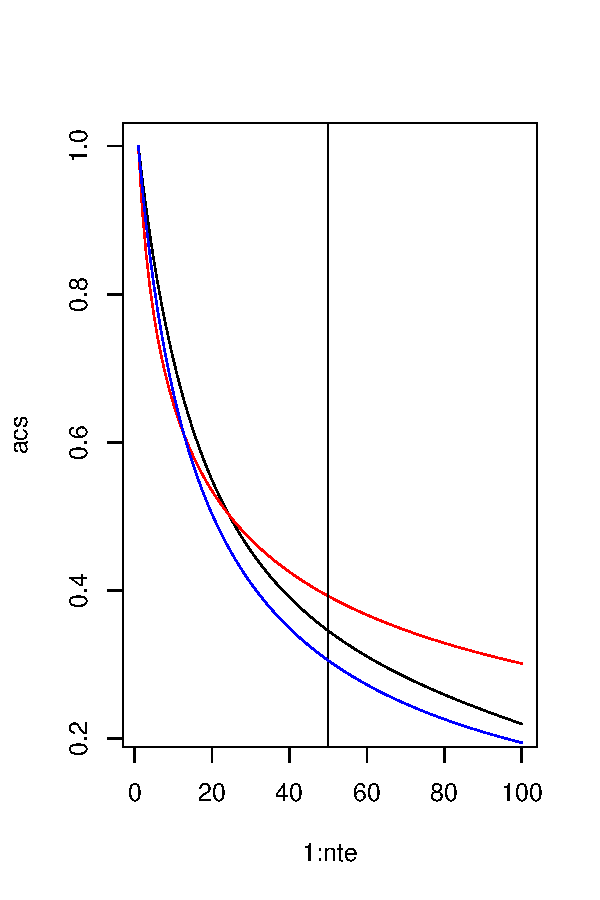
\includegraphics[scale=0.4]{../info_theory_sims/fig_sim5a.pdf} &
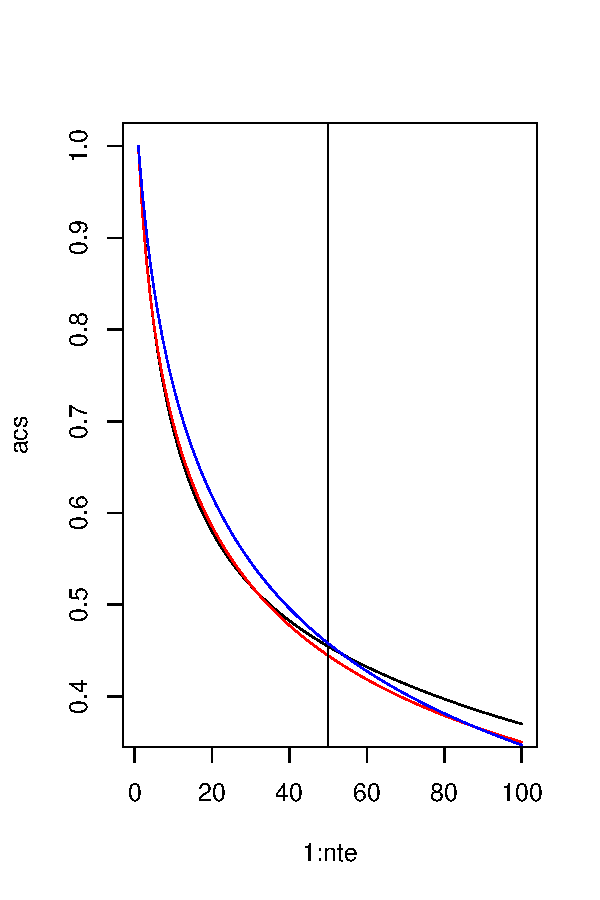
\includegraphics[scale=0.4]{../info_theory_sims/fig_sim5b.pdf} &
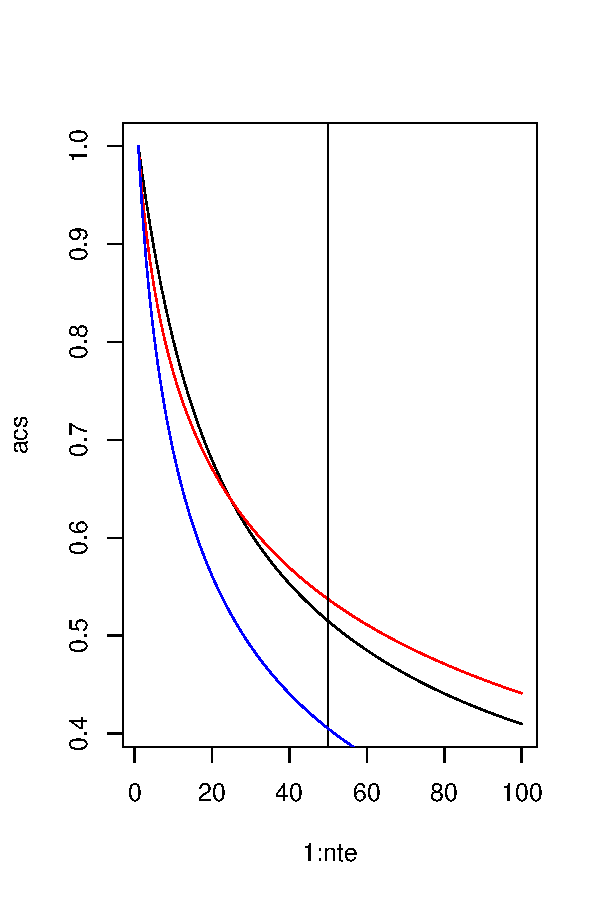
\includegraphics[scale=0.4]{../info_theory_sims/fig_sim5c.pdf}\\
(a) & (b) & (c)
\end{tabular}
\end{center}
\label{fig:simulations}
\caption{Success at recovering identification accuracy curves for various settings.  Black = empirical accuracy curve, Blue = ground truth accuracy curve, Red = estimated accuracy curve. (a) Low-dimensional setting ($n = 20, p = 3, q = 5$).  The estimated accuracy curve is not close to either the empirical curve nor the true accuracy curve.  (b) High-dimensional setting ($n = 2000, p = 30, q = 50$).  The estimated accuracy curve is close to both the empirical and true accuracy curves, and is a better estimate of the true accuracy than the empirical accuracy.  (c) High-dimensional mixture setting. ($n = 2000, p = 30, q = 50$)  Although the estimated curve is similar to the empirical curve, the true accuracy is much diffferent from either.}
\end{figure}

\section{Real-data examples}

Examples using Kay et al data:
\begin{itemize}
\item Comparison of different feature models (subsets of pyramid levels)
\item Comparison of differing voxel numbers
\item Effect of voxel resolution (by averaging neighboring voxels into bigger voxels)
\end{itemize}

\bibliography{neuroinfo}{}
\bibliographystyle{plain}

\end{document}












A common goal in neuroscience experiments is understand how some
aspect of behavior, cognition, or sensation is reflected in brain
activity:




A fundamental challenge of computational neuroscience is to understand
how information about the external world is processed and represented
in the brain.


Each individual neuron aggregates the incoming
information into a single sequence of spikes--an output which is too
simplistic by itself to capture the full complexity of sensory
input. Only by combining the signals from massive ensembles of neurons
is it possible to reconstruct our complex representation of the
world. Nevertheless, neurons form hierarchies of specialization within
neural circuits, which are further organized in various specialized
regions of the brain.  At the lowest level of the hierarchy--individual neurons,
it is possible to infer and interpret the functional relationship between
a neuron and stimulus features of interest using single-cell recording technologies.
Due to the inherent stochasticity of the neural output, it is natural to
view the neuron as a noisy channel, and use mutual information
to quantify how much of the stimulus information is encoded by the neuron.
Moving up the hierarchy to the the macroscale level of organization in the
brain requires both different experimental methodologies and 
new approaches for summarizing and inferring measures of
information in the brain.

Shannon's mutual information $I(X; Y)$ is fundamentally a measure of dependence
between random variables $X$ and $Y$, and is defined as
\[
I(X;Y) = \int p(x, y) \log \frac{p(x, y)}{p(x)p(y)}dxdy.
\]
Various properties of $I(X; Y)$ make it ideal for quantifying the information between
a random stimulus $X$ and the signaling behavior of an ensembles of neurons, $Y$ ~\cite{Borst1999}.
A leading metaphor is that of a noisy communications channel; the mutual
information describes the rate at which $Y$ can communicate bits from
$X$.  This framework is well-suited for summarizing the properties of
a single neuron coding external stimulus information; indeed,
experiments studying the properties of a single or a small number of
neurons often make use of the concept of mutual information in
summarizing or interpreting their results ~\cite{QuianQuiroga2009}. However,
estimating mutual information for multiple channels require large and
over-parameterized generative models.  For instance, one can tractably
estimate mutual information by assuming a multivariate Gaussian model:
however, this approach essentially assumes a linear relationship
between the input and output, and hence fails to quantify nonlinear
dependencies.  As the complexity of stimuli and the number of output
channels increases, these models are hard or impossible to estimate
without gross over-fitting.  As new technologies for simultaneous measurement
of multiple brain regions developed, such as functional MRI, it became
increasingly difficult to quantify information at such scales under the classical approach.
 
Machine learning algorithms showed a way forward: a seminal work
by Haxby (2001) proposed to quantify the information in multiple
channels by measuring how well the stimulus can be identified from the
brain responses, in what is known as ``multivariate pattern analysis''
(MVPA). To demonstrate that a particular brain region responds to a
certain type of sensory information, one employs supervised learning
to build a classifier that classifies the stimulus class from the
brain activation in that region. Classifiers that achieve above-chance
classification accuracy indicate that information from the stimulus is
represented in the brain region. In principle, one could just as well
test the statistical hypothesis that the Fisher information or mutual
information between the stimulus and the activation patterns is
nonzero. But in practice, the machine learning approach enjoys several
advantages: First, it is invariant to the parametric representation of
the stimulus space, and is opportunistic in the parameterization of
the response space. This is an important quality for naturalistic
stimulus-spaces, such as faces or natural images. Second, it scales
better with the dimensionality of both the stimulus space and the
responses space, because a slimmer discriminative model can be used
rather than a fully generative model.

Nevertheless, classification error is problematic for quantifying the
strength of the relation between stimulus and outputs due to its
arbitrary scale and strong dependence on experimental
choices. Classification accuracy depends on the particular choice of
stimuli exemplars employed in the study and the number of partitions
used to define the classes for the classification task. The difficulty
of the classification task depends on the number of classes defined:
high classification accuracy can be achieved relatively easily by
using a coarse partition of stimuli exemplars into classes. In a
meta-analysis on visual decoding, Coutanche et al (2016) quantified
the strength of a classification study using the formula
\[
\text{decoding strength} = \frac{\text{accuracy} - \text{chance}}{\text{chance}}.
\]
Such an approach may compensate for the differences in accuracy due
purely to choice of number of classes defined; however, no theory is
provided to justify the formula. In contrast, mutual information has
ideal properties for quantitatively comparing information between
different studies, or between different brain regions, subjects,
featurization models, or modalities. Not only is the mutual
information defined independently of the arbitrary definition of
stimulus classes (albeit still dependent on an implied distribution
over stimuli), it is even meaningful to discuss the difference between
the mutual information measured for one system and the mutual
information for a second system.

Hence, a popular approach which combines the strengths of the machine
learning approach and the advantages of the information theoretic
approach is to obtain a lower bound on the mutual information by using
the confusion matrix of a classifier.  This is the most popular
approach for estimating mutual information in neuroimaging studies,
but suffers from known shortcomings (Gastpar 2010, Quiroga 2009).
The idea of linking classification performance to mutual information
dates back to the beginnings of information theory: Shannon's original
motivation was to characterize the minimum achievable error
probability of a noisy communication channel.  More explicitly, Fano's
inequality provides a lower bound on mutual information in relation to
the optimal prediction error, or Bayes error.  Fano's inequality can
be further refined to obtain a tighter lower bound on mutual
information (Tebbe and Dwyer 1968.)  However, all approaches to date
can only obtain a lower bound on the mutual information from
classification error.  In practice, the bound obtained may be a vast
underestimate.

In this paper, we propose a new way to link classification performance
to the implied mutual information. 
To create this link we need to overcome the arbitrary choice of
exemplars, and the arbitrary number of classes K.  Towards this end,
we define a notion of $K$-class \emph{average Bayes error} which is
uniquely defined for any given stimulus distribution and stochastic
mapping from stimulus to response.  The $K$-class average Bayes error
is the expectation of the Bayes error (the classification error
of the optimal classifier) when $K$ stimuli exemplars are drawn
i.i.d. from the stimulus distribution, and treated as distinct
classes.  Hence the average Bayes error can in principle be estimated
if the appropriate randomization is employed for designing the
experiment.

Our main theoretical contributions are (i) the derivation of a tight lower bound
on mutual information as a function of $k$-class average Bayes error, and (ii)
the derivation of an asymptotic relationship between the $K$-class average Bayes error and the mutual
information. Although the $K$-class average Bayes error is defined
independently of the particular choice of stimuli, the quantity still
depends on the choice of number of classes, $K$. Mutual information
provides a quantification of information that does not depend on $K$,
allowing more flexible comparisons and easier interpretation. Our
method allows estimates of the $K$-class Bayes error to be translated
into estimate of the mutual information, and this resulting estimator
of mutual information will be asymptotically independent of the choice
of number of classes $K$.




\end{document}





